\documentclass[border=3pt]{standalone}
% Shared preamble for standalone TikZ figures (colors match the slide theme).
\usepackage[T1]{fontenc}
\IfFileExists{sourcesanspro.sty}{\usepackage[default]{sourcesanspro}}{\usepackage[scaled=0.92]{helvet}\renewcommand{\familydefault}{\sfdefault}}
\usepackage{xcolor,tikz}
\usetikzlibrary{arrows.meta,positioning,calc,shapes.geometric,decorations.pathmorphing,decorations.pathreplacing,backgrounds,fit}
\definecolor{fsNavy}{HTML}{1B365D}
\definecolor{fsAccent}{HTML}{C8102E}
\definecolor{fsGold}{HTML}{D39B1E}
\definecolor{fsTeal}{HTML}{1F7A8C}
\definecolor{fsGreen}{HTML}{3A7D44}
\definecolor{fsGray}{HTML}{5B6770}
\definecolor{fsLight}{HTML}{EEF2F6}
\tikzset{
  molbox/.style={draw=black!55,rounded corners=3pt,line width=0.6pt,
                 minimum height=7mm,font=\small\bfseries,inner xsep=3mm},
  site/.style={circle,draw=black!55,fill=white,inner sep=0pt,minimum size=4mm,
               font=\tiny\bfseries,line width=0.5pt},
  psite/.style={site,fill=fsAccent,text=white},
  bond/.style={line width=1.3pt,black!70},
  callout/.style={font=\scriptsize,text=fsGray,align=left},
  pointer/.style={-{Stealth[length=1.6mm]},fsGray,line width=0.5pt},
}
\newcommand{\code}[1]{{\ttfamily #1}}

\begin{document}
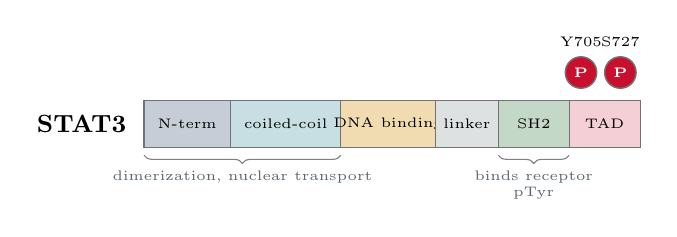
\begin{tikzpicture}[x=1cm,y=1cm]
  \foreach \xa/\wa/\col/\lab in {0/1.1/fsNavy!25/N-term, 1.1/1.4/fsTeal!25/coiled-coil,
                           2.5/1.2/fsGold!35/DNA binding, 3.7/0.8/fsGray!20/linker,
                           4.5/0.9/fsGreen!30/SH2, 5.4/0.9/fsAccent!20/TAD}
    {\draw[black!55,fill=\col] (\xa,0) rectangle ++(\wa,0.6);
     \pgfmathsetmacro{\xm}{\xa+\wa/2}
     \node[font=\tiny,align=center] at (\xm,0.3) {\lab};}
  \node[psite] (y) at (5.55,0.95) {P};
  \node[font=\tiny,above=0pt of y] {Y705};
  \node[psite] (s) at (6.05,0.95) {P};
  \node[font=\tiny,above=0pt of s] {S727};
  \node[font=\small\bfseries,anchor=east] at (-0.1,0.3) {STAT3};
  \draw[decorate,decoration={brace,mirror,amplitude=3pt},black!50] (0,-0.1) -- (2.5,-0.1)
    node[midway,below=2pt,font=\tiny,text=fsGray] {dimerization, nuclear transport};
  \draw[decorate,decoration={brace,mirror,amplitude=3pt},black!50] (4.5,-0.1) -- (5.4,-0.1)
    node[midway,below=2pt,font=\tiny,text=fsGray,align=center] {binds receptor\\pTyr};
\end{tikzpicture}
\end{document}
